% rubber: module pdftex
% rubber: module index
% rubber: module xr
\documentclass[a4paper,american,12pt]{scrreprt}

\usepackage[margin=1.5cm]{geometry}

\usepackage{graphicx}
\usepackage[headsepline]{scrpage2}
\usepackage[utf8]{inputenc}
\usepackage[T1]{fontenc}
\usepackage{color}
\usepackage{caption}

\usepackage{subcaption}

%\usepackage{times}
%\usepackage{lmodern}
\usepackage{mathptmx}
% required for mathbb
\usepackage{amsmath}
%\usepackage{courier}

\usepackage{txfonts}
%\usepackage[scaled=.9]{helvet}

\usepackage{babel}
\usepackage{microtype}

\usepackage{listings}

\usepackage[hyperfootnotes=false,hidelinks]{hyperref}

\usepackage{todonotes}
\usepackage{xspace}

\usepackage{gitinfo}

\usepackage{placeins}

\usepackage{tikz}
\usetikzlibrary{shadows}

\automark[section]{chapter}

\parskip.5em
\parindent0em

\newcommand{\cinco}{\textsc{Cinco}\xspace}
\newcommand{\code}[1]{\texttt{#1}}
\newcommand{\key}[1]{\mbox{[#1]}}
\newcommand{\newnotion}[1]{\emph{#1}}
\newcommand{\gui}[1]{\flqq{}\textsf{#1}\frqq{}}
\newcommand{\mgl}[1]{\raisebox{-0.05em}{\mbox{
\includegraphics[height=0.7em]{icons/mgl_icon.pdf}}\kern 0.2em \code{#1}}}
\newcommand{\msl}[1]{\raisebox{-0.05em}{\mbox{
\includegraphics[height=0.7em]{icons/msl_icon.pdf}}\kern 0.2em \code{#1}}}

% Thanks to Thorsten Donig for the nice keystroke visualization
% https://tex.stackexchange.com/questions/5226/keyboard-font-for-latex#5227
\newcommand{\keystroke}[1]{%
  \raisebox{0.15em}{
  \tikz[baseline=(key.base)]
    \node[%
      draw,
      fill=white,
      drop shadow={shadow xshift=0.25ex,shadow yshift=-0.25ex,fill=black,opacity=0.75},
      rectangle,
      rounded corners=2pt,
      inner sep=1pt,
      line width=0.5pt,
      font=\scriptsize\sffamily
    ](key) {\ #1\ \strut}
  ;
  }
  \kern -0.25em
}

\definecolor{numbergray}{gray}{0.5}

\lstdefinestyle{mgl}{
   %language=XML,
   columns=fixed,
	breaklines=true,
	numbers=left,
	numberstyle=\tiny,
	stepnumber=1,
	numbersep=5pt,
   showspaces=false,
   showstringspaces=false,
   frame=tblr,
   tabsize=2,
   frame=shadowbox,
   columns=fixed,
   basicstyle=\ttfamily\scriptsize,
   %basicstyle=\scriptsize,
   rulesepcolor=\color[rgb]{0.6, 0.6, 0.6},
   %keywordstyle=\color[rgb]{0.5,0,0.4}\textbf, 
    keywordstyle=\color[rgb]{0.5,0,0.34}\textbf,
   %keywordstyle=\color[rgb]{0.5,0,0.4}\bfseries, 
   %keywordstyle=\color[rgb]{0.5,0,0.4},
   stringstyle=\color{blue},
   commentstyle=\color[rgb]{0.4,0.7,0.4},
   backgroundcolor=\color[rgb]{0.97,0.97,0.97},
   morekeywords={node, edge, attr, container, as, package, nsURI, iconPath, diagramExtension, graphModel, incomingEdges, outgoingEdges},
	morestring=[b]",
   showtabs=false,
	morecomment=[l]{//},
	morecomment=[s]{/*}{*/},
   literate={0}{{{\color{numbergray}0}}}{1}%
		{1}{{{\color{numbergray}1}}}{1}%
		{2}{{{\color{numbergray}2}}}{1}%
		{3}{{{\color{numbergray}3}}}{1}%
		{4}{{{\color{numbergray}4}}}{1}%
		{5}{{{\color{numbergray}5}}}{1}%
		{6}{{{\color{numbergray}6}}}{1}%
		{7}{{{\color{numbergray}7}}}{1}%
		{8}{{{\color{numbergray}8}}}{1}%
		{9}{{{\color{numbergray}9}}}{1}
}

\newcommand{\includemgl}[3]{\lstinputlisting[style=mgl, float=tb, caption=#2, label=#3, captionpos=b]{#1}}


\lstdefinestyle{style}{
   %language=XML,
   columns=fixed,
	breaklines=true,
	numbers=left,
	numberstyle=\tiny,
	stepnumber=1,
	numbersep=5pt,
   showspaces=false,
   showstringspaces=false,
   frame=tblr,
   tabsize=2,
   frame=shadowbox,
   columns=fixed,
   basicstyle=\ttfamily\scriptsize,
   %basicstyle=\scriptsize,
   rulesepcolor=\color[rgb]{0.6, 0.6, 0.6},
   keywordstyle=\color[rgb]{0.5,0,0.4}\textbf, 
   %keywordstyle=\color[rgb]{0.5,0,0.4}\bfseries, 
   %keywordstyle=\color[rgb]{0.5,0,0.4},
   stringstyle=\color{blue},
   commentstyle=\color[rgb]{0.4,0.7,0.4},
   backgroundcolor=\color[rgb]{0.97,0.97,0.97},
	morekeywords={nodeStyle, edgeStyle, rectangle, ellipse, roundedRectangle,
	text, polyline, size, corner, position, value, color, lineStyle, lineWidth,
	SOLID, DASH, DASHDOT, DASHDOTDOT, DOT, decorator, location, relativeToMid,
	points, appearance, appearanceProvider, background, foreground, relativeTo,
	ARROW, CIRCLE, TRIANGLE, CENTER, MIDDLE, @, extends},
	morestring=[b]",
   showtabs=false,
	morecomment=[l]{//},
	morecomment=[s]{/*}{*/},
   literate={0}{{{\color{numbergray}0}}}{1}%
		{1}{{{\color{numbergray}1}}}{1}%
		{2}{{{\color{numbergray}2}}}{1}%
		{3}{{{\color{numbergray}3}}}{1}%
		{4}{{{\color{numbergray}4}}}{1}%
		{5}{{{\color{numbergray}5}}}{1}%
		{6}{{{\color{numbergray}6}}}{1}%
		{7}{{{\color{numbergray}7}}}{1}%
		{8}{{{\color{numbergray}8}}}{1}%
		{9}{{{\color{numbergray}9}}}{1}
}

\newcommand{\includestyle}[3]{\lstinputlisting[style=style, float=tb, caption=#2, label=#3, captionpos=b]{#1}}


\lstdefinestyle{java}{
   language=Java,
   breaklines=true,
   numbers=left,
   numberstyle=\tiny,
   stepnumber=1,
   numbersep=5pt,
   showspaces=false,
   showstringspaces=false,
   frame=tblr,
   tabsize=2,
   frame=shadowbox,
   columns=fixed,
   %basicstyle=\ttfamily\small,
   basicstyle=\ttfamily\scriptsize,
   rulesepcolor=\color[rgb]{0.6, 0.6, 0.6},
   %keywordstyle=\color[rgb]{0.5,0,0.4}\bfseries, 
   keywordstyle=\color[rgb]{0.5,0,0.4},
   stringstyle=\color{blue},
   commentstyle=\color[rgb]{0.4,0.7,0.4},
   backgroundcolor=\color[rgb]{0.97,0.97,0.97},
   showtabs=false
}

\newcommand{\includejava}[3]{\lstinputlisting[style=java, float=tb, caption=#2, label=#3, captionpos=b]{#1}}


\begin{document}

\title{\cinco User's Manual}
\author{Stefan Naujokat}
\date{\today}

\begin{titlepage}

\vspace*{3cm}

\makebox[2.5cm]{}
\begin{minipage}{8.0cm}
\begin{center}
	{\huge\bfseries \cinco{} User's Manual}

	\vspace{1.5em}

	{\large Stefan Naujokat}

	\vspace{1.5em}

	{\large (version id: \gitAbbrevHash{})}
\end{center}
 \end{minipage}

\vspace{-4em}

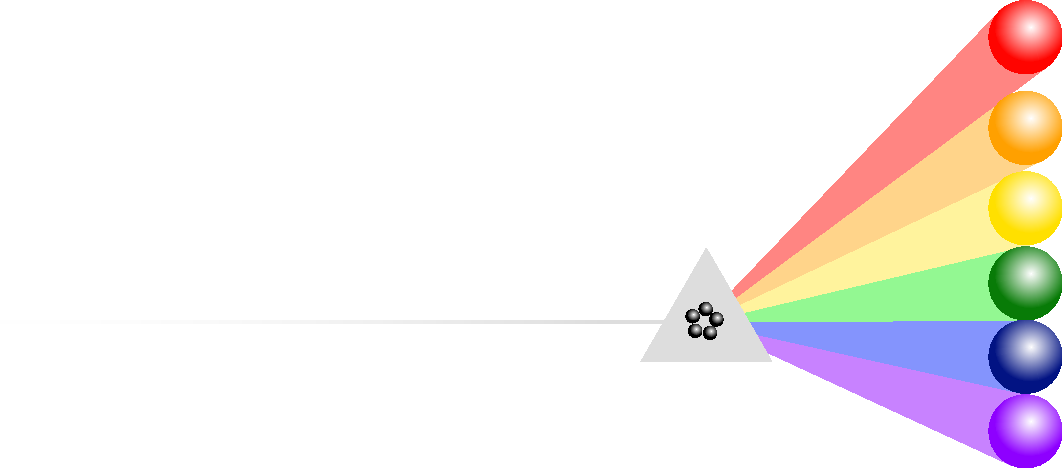
\includegraphics[width=0.8\textwidth]{figures/cinco-logo.pdf}

\vfill
\end{titlepage}


\chapter{Basics}

\section{About This Document}

This is the technical manual for the ``\cinco SCCE Meta Tooling Suite'' (in
short just \cinco). It is intended to provide a basic usage introduction as
well as (coming soon) reference for all features and keywords. It only implicitely covers the
conceptual ideas behind \cinco. For a more in-depth and scientific view on those,
please refer to the following publications:
%
\begin{itemize}
%\item S. Naujokat et al.: Full generation of domain-specific graphical modeling tools: a
%meta$^2$modeling approach \cite{NaLSKM2014}
\item S. Naujokat et al.: Domain-Specific Code Generator Modeling: A Case Study for
Multi-Faceted Concurrent Systems \cite{NaTISL2014}
\item D. Kopetzki: Model-based generation of graphical editors on
the basis of abstract meta-model specifications \cite{Kopetz2014}
\end{itemize}

This document will constantly be revised and extendend. The latest version will
always be available for download at \url{http://cinco.scce.info/resources/}. 

\begin{description}
\item[covered version] \cinco v. 0.6
\item[git commit id] \gitAbbrevHash{}
\item[date of build] \today
\end{description}

\section{Introduction}

The ``\cinco{} SCCE Meta Tooling Suite'' is an integrated devlopment environment
(IDE) for the quick and easy development of domain-specific graphical modeling
tools. \cinco{} makes use of several frameworks from the Eclipse Modeling
Project, but its main goal is to hide those frameworks' intricacy from the
tool developer. \cinco{} provides three simple textual specification languages (MGL,
MSL, and CPD, see below) for the high-level characterization of the developed tool's
structural and visual features. Above that, \cinco{} is also a full Java IDE, so
that the portions of the developed tool that are not described in a declarative
way can seamlessly be developed in the same environment.

Crucial to \cinco is the concept of code generation. Much of the code of a
modeling tool that is developed with \cinco (in the following called \cinco
Product, or just CP) is generated automatically from abstract specifications,
such as the already mentioned MGL, MSL and CPD files. It is of utmost importance
that you \emph{never} make any changes to automatically generated
code\footnotemark{}, as all those changes will be gone once the code generation
is run again.

\footnotetext{Of course, this does not apply to automatically generated 'source'
files (such as examples and templates). Those are generated for convenience to
have a basic version to start working on.}

\section{Download \& Installation}

As \cinco{} is a full Eclipse-based IDE including the Eclipse Modeling Tools
(EMF, Xtext, Graphiti, etc.) and the Java Development Tooling (JDT) in addition
to our own plug-ins the download size is almost 300 MB. We are planning to
provide the \cinco{}-specific plug-ins via an Eclipse update site in the future,
but for now you need to download the whole package as one.

Please note: \cinco{} itself is developed under the ``Eclipse Public License v. 1.0'', 
but the executable build contains several libraries from the jABC
project, for which the following license applies:

\begin{verbatim}
===============================================================================
This software is free to use.

You are not allowed to redistribute, modify or decompile this software.

Third-party components are included for which these restrictions may not apply.
Please refer to the documentation for details.

THIS SOFTWARE IS PROVIDED ``AS IS'' AND WITHOUT ANY EXPRESS OR IMPLIED
WARRANTIES, INCLUDING, WITHOUT LIMITATION, THE IMPLIED WARRANTIES OF
MERCHANTIBILITY AND FITNESS FOR A PARTICULAR PURPOSE.
===============================================================================
\end{verbatim}

\cinco{} requires OpenJDK 7 to be installed on your system as main Java
installation (i.e. JAVA\_HOME pointing there). Apart from that, you just have to
choose the correct zip file for download (Linux/Window/Mac in 32 or 64 bit
variant), unzip it and execute the included binary: \code{cinco} for Mac and
Linux, \code{cinco.exe} for Windows.

\section{Getting Started Tutorial}

\subsection{Launching \cinco for the First Time}
\label{sec:firstLaunch}

When launching \cinco{} it will first query you for the location of a workspace
directory. Choose some place on your harddisk that is not within the \cinco
installation folder. This workspace will contain all your \cinco projects
and the according metadata, as well as sub-projects, specification files, source
code etc. It is possible to use different workspaces (e.g. for different
projects). If you don't want to use multiple ones for now, you can check
\gui{Use this as default and do not ask again} before clicking \gui{OK}.

\begin{figure}
	\centering
	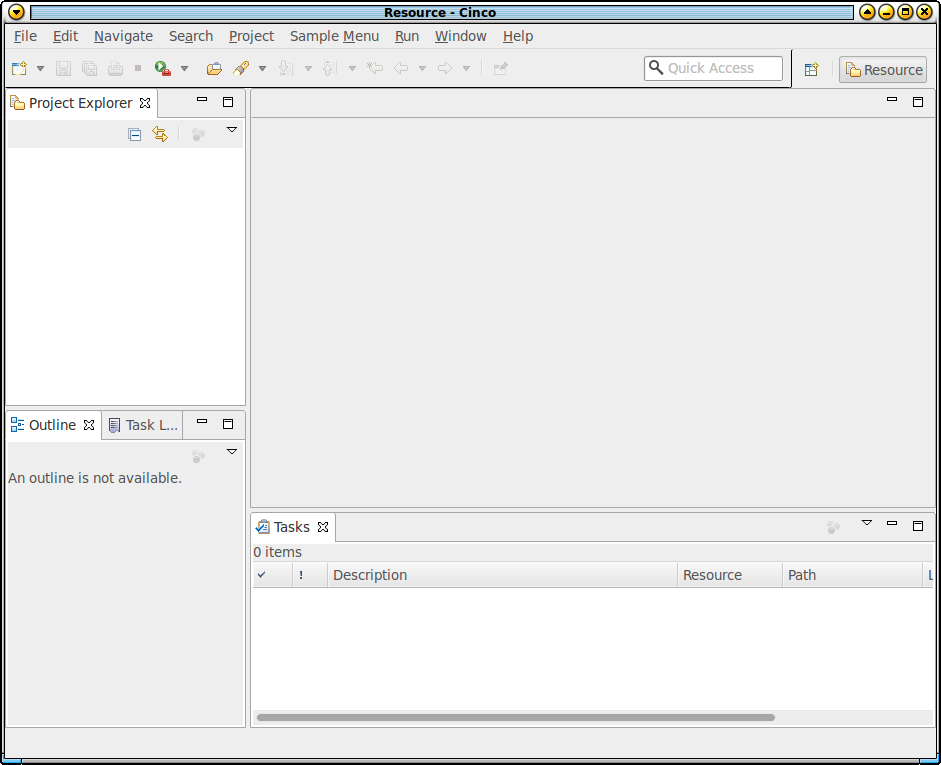
\includegraphics[width=.7\textwidth]{screenshots/cinco-gui-firststart.png} 
	\caption{First startup should look like this}
	\label{fig:firstStart}
\end{figure}

After choosing the workspace \cinco should start and look like
Fig.~\ref{fig:firstStart}. The GUI is partitioned into so-called
\newnotion{Views}. For now, the \gui{Project Explorer} and the editor area (the
big empty grey space on the right) are the most important ones. 

\subsection{Creating a \cinco Product Project}
\label{sec:wizard}

\begin{figure}
	\centering
	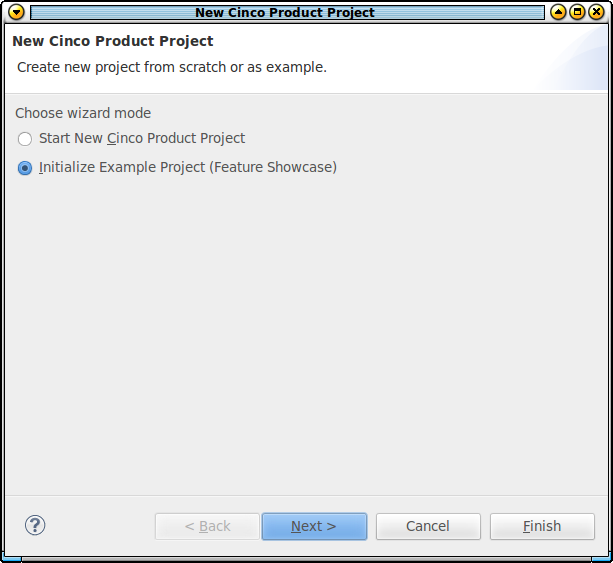
\includegraphics[width=.5\textwidth]{screenshots/new-cp-wizard.png}
	\caption{Use the wizard to create a new example project}
	\label{fig:cpWizard}
\end{figure}

To get a new \newnotion{Cinco Product} project initialized, we'll now use the
built-in wizard to create some example files to start working with.
Right-click somewhere within the \gui{Project Explorer} and choose \gui{New / Cinco Product
Project}. The wizard as depicted in Fig.~\ref{fig:cpWizard} appears. The wizard
has two modes. You can either start a completely new project from scratch or
generate an example project showing off some of the \cinco{} features. We'll go for
the latter one for now. Select \gui{Initialize Example Project (Feature
Showcase)} and hit \gui{Next}. 

\begin{figure}
	\centering
	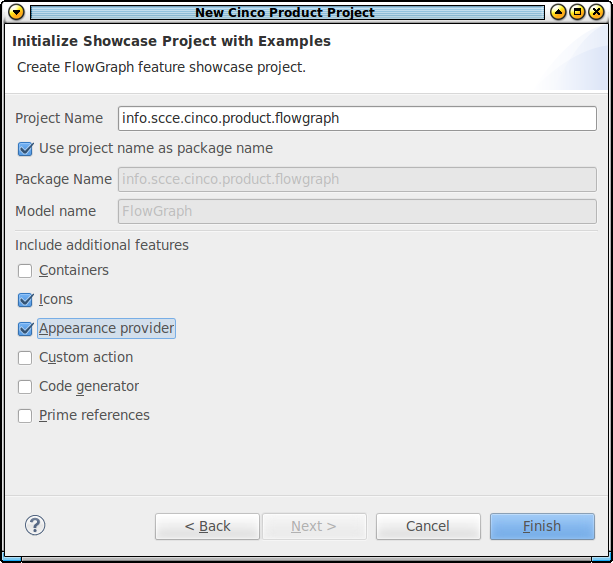
\includegraphics[width=.5\textwidth]{screenshots/new-cp-wizard2.png}
	\caption{Select example features that shall be generated}
	\label{fig:cpWizard2}
\end{figure}

The next page of the wizard now lets you configure some basic things for your
example project (cf. Fig.~\ref{fig:cpWizard2}). Please note that the model name
is fixed, as the generated example is a flow graph. For now, you probably should leave
the project/package name as suggested; if you create additional examples with
the wizard later, you can choose different names here to distinguish them. Each
feature you select at the bottom will generate additional parts in the example.
We suggest to use \gui{Icons} and \gui{Appearance provider} to keep the files
manageable small for your first attempt using \cinco{}. Confirm your
selection with \gui{Finish}

\begin{figure}
	\centering
	\begin{subfigure}[t]{0.40\textwidth}
		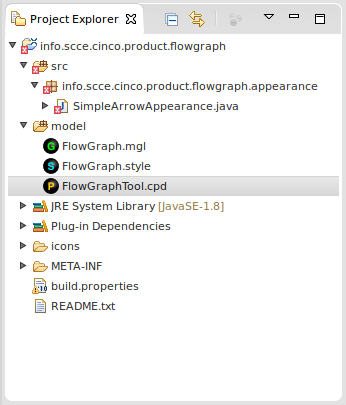
\includegraphics[width=\textwidth]{screenshots/example-cp-pregen.png}
		\caption{Project after running the wizard}
		\label{fig:cpPreGen}
	\end{subfigure}
	\qquad
	\begin{subfigure}[t]{0.40\textwidth}
		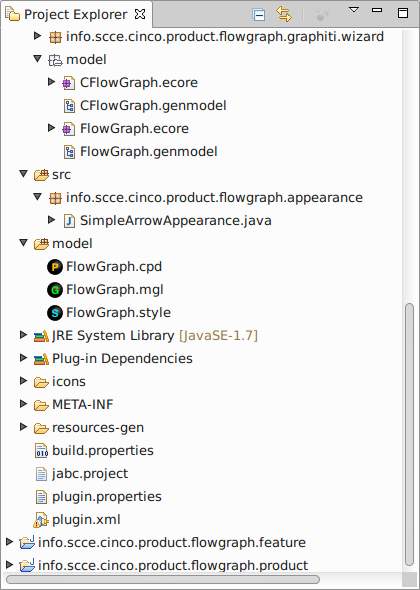
\includegraphics[width=\textwidth]{screenshots/example-cp-postgen.png}
		\caption{Project after code generation}
		\label{fig:cpPostGen}
	\end{subfigure}
	\caption{Project file system view before and after \cinco{} product generation}
\end{figure}

After running the wizard, the project explorer contains your freshly created
project. Depending on the names you've chosen, it should now look somewhat
similar to Fig.~\ref{fig:cpPreGen}. Please note that the compile error marked at
\code{SimpleArrowAppearance.java} is not unexpected. The Java class refers to
other Java entities that have not yet been generated. 

You might want to take a short look into those initialized files (especially the ones in the
\code{model} folder), but before we delve more deeply
into their contents (which we will do
in Sec.~\ref{sec:examplefiles}), let's first generate this example CP and give
it a try. Just right-click on the \cpd{FlowGraph.cpd} and
choose \gui{Generate Cinco Product}. Shortly after, your project explorer should
look like Fig.~\ref{fig:cpPostGen}. Several new files, directories, and
projects -- which will be even more once you start using advanced
features of \cinco{}, such as meta plug-ins -- have been generated. Also, the
compile error we've noticed before is gone. 

Whenever you change the CP's specification files, you need to re-generate the
code. Previously generated code (i.e. everything that is in a *-gen folder and
all generated projects) will be deleted on re-generation. But as you never do
any manual changes to the generated code, this is no problem. 

\subsection{Testing the \cinco Product} \label{sec:testing}

Now, let's test the tool we just generated. Within the project explorer,
right-click on the root folder of your main project and choose \gui{Run As /
Eclipse Application}. You should now see the \cinco splash screen again,
starting a different Eclipse product: your modeling tool. \footnotemark

\footnotetext{Please note: When you use the here presented 'simple way' of
starting your product (via the \gui{Run As} menu) you will actually start your
tool including \emph{all} the \cinco plug-ins and libraries. In fact, you start
a second \cinco enriched with the new features we just generated. In the long run, this 
not what is desired, because a tool developer needs to work with different tools
than the tool user. You might have noticed the new .product project. This
is a generated Eclipse product definition that provides an easy way of exporting your
tool with an own branding (splash screen, icons, etc.) into a standalone
application. For testing purposes, however, the easy way should be favored, as
it does not impose any obstacles other than ample unnecessary GUI elements.}

Again, you should see an empty tool like Fig.~\ref{fig:firstStart}. To create a
new model we first need a new project where it can be placed. This time,
however, we don't need a \cinco product project (as we don't want to develop
another \cinco product within the just started \cinco product). A plain project
is enough this time. Right-click somewhere in the project explorer and select
\gui{New / Project... / General / Project / Next >}, give the project some name
and click \gui{Finish}. Then, right-click on your newly created project and
select \gui{New / Other... / Cinco Product / New FlowGraph} to create your
first CP-specific model.

The editor area now shows your empty model with a drawing grid. On the right
side you see a \gui{Palette}, containing the elements you can now use for modeling.
The elements you see there are in the \gui{Palette / Objects}
category: \code{Start}, \code{End}, and \code{Activity}. Those are the three node
types that are were automatically included in the \mgl{FlowGraph.mgl} by the
wizard. Begin modeling by just drag\&dropping a few different nodes into the
modeling area. To connect nodes, you can just hover over one and drag the small
appearing arrow icon onto another one. For the \code{Activity} node type and
the edges originating from them, you can use the \gui{Properties} view (bottom
of your window) to set attributes; \code{Name} and \code{Description} for the
node as well as \code{Label} for the edge. An activity's name is displayed
within the node shape (the blue box) and the edge label is shown as a floating
(and movable) textbox next to the edge. Fig.~\ref{fig:firstModel} shows an
example how your tool should look now.

\begin{figure}
	\centering
	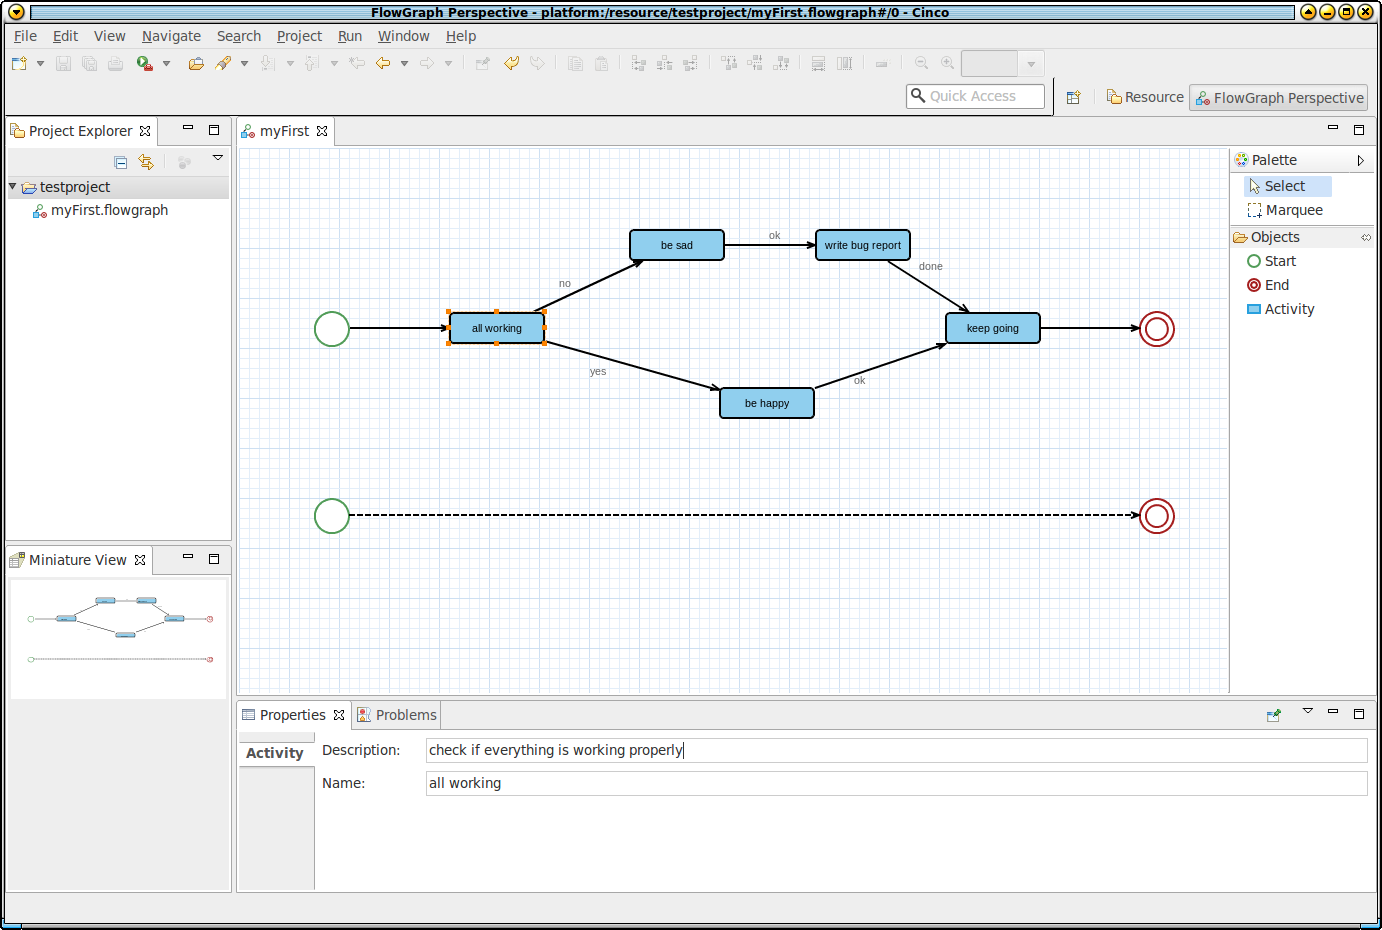
\includegraphics[width=.9\textwidth]{screenshots/cp-first-model.png} 
	\caption{The first model that was modeled using the example \cinco product}
	\label{fig:firstModel}
\end{figure}

The modeling elements abide by the following syntactic rules:

\begin{itemize}
\item \code{Start} nodes (green circle) have at most one outgoing edge of type
	\code{Transition}, but no incoming edges.
\item \code{End} nodes (double red circle) have arbitrarily many incoming edges,
	but no outgoing.
\item \code{Activity} (blue box) nodes have multiple outgoing edges of type
	\code{LabeledTransition}, and may have multiple incoming edges of both types.
	The attribute \code{Name} is displayed centered within the box.
\item \code{LabeledTransition} edges connect \code{Activity} nodes to arbitrary other nodes and
	have their attribute \code{Label} displayed as movable caption next to it.
\item \code{Transition} edges only originate from \code{Start} nodes. If such an
	edge directly leads to an \code{End} node, it is displayed with a dashed
	line.
\end{itemize}

Those rules are all defined within the example \cinco specification files that
were created by the wizard. The next section will therefore provide a detailed
discussion on the contents of those files.

\section{Discussion on the Example Files}
\label{sec:examplefiles}

We consider our specification formats MGL, MSL, and CPD fairly self-explanatory,
meaning that one usually can understand most of their contents without detailed
knowledge on available keywords or syntactic structures. This section
will nonetheless detail on our two example files, but you might want to have a look at
your \mgl{FlowGraph.mgl}, \msl{FlowGraph.style}, and \cpd{FlowGraph.cpd} beforehand, to decide for
yourself. 

However, writing (instead of just understanding) a programming or specification language usually is a totally
different matter. But here, \cinco heavily benefits from being implemented
with libraries from the Eclipse Modeling Project, in this case especially Xtext:
The so-called \newnotion{Content Assist} that is generated for every Xtext-based
editor provides a very useful autocompletion when
\keystroke{Ctrl}+\keystroke{Space} is pressed (if you ever programmed Java using
Eclipse, you most likely know this shortcut already). With this feature it is
often not even required to read the documentation, as one can autocomplete
through the whole specification file, manually inserting an identifier every now and
then.

Modeling tool development with \cinco centers around two textual specification
files. On the one hand we have a file in the ``Meta Graph Language'' (MGL) that
contains the structural information on the tool's model. On the other hand, a
``Meta Style Language'' (MSL) file\footnotemark{} is required to specify the
visual characteristics (e.g.  shapes and colors) of this model. The third
specification format is the ``\cinco Product Definition'' (CPD), which is the
entry point for the generation. In it, (potentially) multiple MGL files can be
given that are generated in one sweep. The following
subsections will each provide an introduction to one of this specification
languages alongside the example files created by the new project wizard.

\footnotetext{Please note that the file extension for MSL is currently
\code{.style}. We are planning to change this to \code{.msl} in a future
release.}

\subsection{MGL File} \label{sec:mgl} 

\includemgl{listings/FlowGraph.mgl}{FlowGraph MGL file}{lst:myMGL}

Listing \ref{lst:myMGL} shows the \mgl{FlowGraph.mgl} as it was initialized in
Sec.~\ref{sec:wizard}. Aside from some general configuration stuff in lines
1-7 and an attribute declaration in line 9, it contains three two different kinds of modeling component declaration:
\begin{itemize}
\item Node type definitions (3x)
\item Edge type definitions (2x)
\end{itemize}

Each of those \kw{node} \code{\{...\}} or \kw{edge} \code{\{...\}} blocks can be preceeded
by a varying number of annotations (starting with the @-symbol). Also following
the syntax of Java, everything from \code{//} to the end of the line is ignored
(single line comment), as well as everything from \code{/*} to \code{*/}
(multi-line comment).

\subsubsection{Node Types}

Each node type defines one kind of component that can be inserted into the
graphModel by drag\&dropping it from the \gui{Palette} into the modeling area.
Doing so will create a dedicated instance of this node type, so that attributes
(like name or description in the Activity node, cf. lines 36 and 37) can be set
seperately for each occurance in the model.

Node types can declare an arbitrary amount of such attributes. An attribute's
name (written after the keyword \kw{as}) is displayed as a label next to the
editing field in the \gui{Properties View}. Possible data types for attributes
(written directly after the keyword \kw{attr}) are currently \code{EString},
\code{EInt}, \code{EDouble} and enumerations defined within the MGL (not in this
example). There is also basic support to reference instances of the other node
types from the same MGL. However, this node type currently needs a \code{name} attribute
that will be displayed in a dropdown box when choosing the referenced node.

The definition how the different node types can be connected using edges is
done with the \kw{incomingEdges} and \kw{outgoingEdges} keywords\footnotemark{}.
%
\footnotetext{Earlier versions of \cinco{} used the dual representation of
defining \kw{targetNodes} and \kw{sourceNodes} in the edge type. However, this did
not allow for the declaration of cardinalities.}
%
Enclosed in parantheses you can express a comma-seperated list of constraints,
each suffixed by an upper/lower bound range in brackets. Line 39 shows a 
declaration of outgoing edges using one such contraint. It states that at least
one LabeledTransition has to originate from every Activity node. The \code{*}
that is used as upper bound means "infinity" (i.e. arbitrarily many). If a set
of multiple edge types shall be defined per constraint -- meaning that any
element from the set can be used -- they can be explicitely enumerated
in curly brackets. Line 29 shows one such set constraint. It expresses that each
End node needs at least one incoming edge of the type Transition or of the type
LabeledTransition. As there are only those two edge types in our example, this
is equivalent to the wildcard expression \code{(*[1 ,*])}

Node types can have an \code{@icon} annotation to specify an image that will be
displayed in the tool palette next to the type name (cf. Fig.
\ref{fig:firstModel}). The parameter can either be a path relative to the MGL
project, as used within our example (lines 12, 19 and 34), or a so-called
platform URI which for instance allows to reference files in other bundles. The
relative path from line 12 would look like this in absolute notation:

\code{@icon("platform:/resource/info.scce.cinco.product.flowgraph/icons/Start.png")}

\FloatBarrier

Finally, the \code{@style} annotation is used to assign a node style from the
MSL definition to this node. The first parameter must equal the style identifier
(following after the \kw{nodeStyle} keyword, see Sect.~\ref{sec:msl}). After
that, a list of further parameters may follow, which can be used to pass the
runtime value of attributes to the style. For example, for the Activity node
(cf. line 33) the current value of the attribute "name" is passed and displayed
as text in the center of the style "blueTextRectangle". If the description
attribute needed to be passed as well, the line would look like this:

\code{@style (blueTextRectangle, "\$\{name\}", "\$\{description\}")}

It is not mandatory to establish a one-to-one relation between nodes and styles
like it is done in the generated example. Multiple nodes can use the same style 
and, for instance, pass different attributes. However, depending on the domain
the \cinco product is developed for, it might be a good idea to be able to
visually distinguish the different node types.


\subsubsection{Edge Types}

Edge type declarations are similar to node type declarations. Or more precisely,
they allow a subset of the nodes' features: multiple attributes can be defined
and a style is given with the \code{@style} annotation (though this time of
course an edge style, not a node style, is referenced).

\begin{figure}[h]
	\centering
	\begin{subfigure}[t]{0.30\textwidth}
		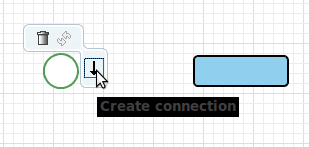
\includegraphics[width=\textwidth]{screenshots/connect1.png}
		\caption{Hover over node}
		\label{fig:connect1}
	\end{subfigure}
	\quad
	\begin{subfigure}[t]{0.30\textwidth}
		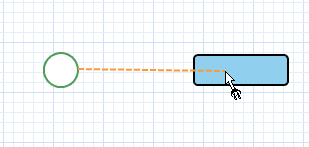
\includegraphics[width=\textwidth]{screenshots/connect2.png}
		\caption{Drag connect icon to target}
		\label{fig:connect2}
	\end{subfigure}
	\quad
	\begin{subfigure}[t]{0.30\textwidth}
		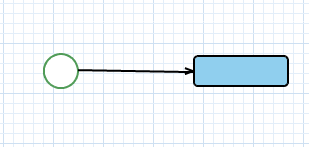
\includegraphics[width=\textwidth]{screenshots/connect3.png}
		\caption{Done}
		\label{fig:connect3}
	\end{subfigure}
	\caption{Creating a new edge using the connect tool that appears when
	hovering a node}
	\label{fig:connect}
\end{figure}

The major difference is that in the running \cinco product the edge types are
not inserted by selecting the corresponding tool from the palette, but by
drag\&dropping a connect icon that appears when hovering over a node onto a
target node. In case multiple edge types are possible (not in the generated
example), you will be queried to choose one after releasing the mouse button on
the target node.

\subsubsection{GraphModel Type}

Prior to the definition of node and edge types\footnote{Actually, the \kw{node}
and \kw{edge} blocks are located \emph{in} this \kw{graphModel} block. See
Listing \ref{lst:myMGL}.} some global things can be specified for your \cinco
product's model type using a \kw{graphModel} \code{\{...\}} block.  This time,
the \code{@style} annotation points to your \msl{FlowGraph.style}, but
attributes are defined identically as for nodes and edges.

The \kw{package} declaration defines the Java package name that should be used
as base package for all generated classes and packages. If you browse the
generated source files in your main project and the other generated ones, you'll
notice that every package is prefixed with the one defined here. While this is
intended to provide "unique" fully qualified names in the Java world, the
\kw{nsURI} keyword defines the unique identifier for the generated Ecore
metamodel.

The \kw{diagramExtension} keyword determines the file extension that will be
used for your models and, last but not least, an icon file for those model can
be defined using the \kw{iconPath} keyword. It will be used on several occasions
in the final product, but most importantly to highlight your created models in
the \gui{Project Explorer} (cf. Fig. \ref{fig:firstModel}) 

\subsection{MSL File} \label{sec:msl}

\includestyle{listings/FlowGraph.style}{FlowGraph MSL file}{lst:myMSL}

Listing \ref{lst:myMSL} shows the \msl{FlowGraph.style} as it was initialized
in Sec.~\ref{sec:wizard}. It consists of appearances, node styles, and
edge styles, which will individually be discussed in the following paragraphs.

\subsubsection{Appearances}

Appearances are used to group some basic visual attribues (such as colors,
fonts, or line width and style) under one name, so that it can be referenced by
the other graphical elements. They are primarily defined using an
\kw{appearance} \code{\{...\}} block. For instance, lines 1-4 define an
appearance named "default" that sets the background color to some light blue and
the line width to 2 pixels. Colors are RGB values, but for convenience
\keystroke{Ctrl}+\keystroke{Space} can be used to open a special color chooser
window.

The keyword \kw{extends} allows to inherit the values from another appearance
and add/overwrite selected ones (cf. line 6). Also, \newnotion{inline
appearances} are supported: Wherever an appearance can be set (cf.
node/edge styles below), an unnamed \kw{appearance} block can be inserted to
directly specify those values. Such an inline appearance can also inherit from
a named one using the keyword \kw{extends} (cf. line 25).

Furthermore, it is sometimes necessary to change the appearance of a graphical
element subject to some information that is only available at runtime. This
could, for instance, be a second cirlce to identify accepting states in a state
diagram. Also, the different appearances of the \code{Transition} edge, depending
on whether it is connected to an \code{End} node or an \code{Activity} node (as
discussed in Sec.~\ref{sec:testing}), requires the appearance not to be static. 

For such cases, \cinco{} supports \newnotion{dynamic appearance providers},
which are special Java classes implementing the \code{StyleAppearanceProvider}
interface and whose \code{getAppearance} method is called at runtime to
determine the current appearance of the element. They are referenced in MSL using
the \kw{appearanceProvider} keyword (cf. line 49).


\subsubsection{Node Styles}

Each node style is defined using a \kw{nodeStyle} \code{\{...\}} block and
consists of at least one primary \newnotion{shape} declaration. For example, the
"greenCircle" style (lines 23-31) consists of a single \kw{ellipse} shape with
width and height of 36 pixels (making it a circle) and an
inline appearance that extends the appearance "default". If the primary shape is
a \newnotion{container shape}, additional child shapes can be included, which is
done for the style "redCircle" (cf. lines 15-19). To allow relative positioning
of child shapes, shapes can be given an identifier that need to be placed after
the respective keyword. In the "redCircle" style the primary shape is named
"outer" (cf. line 12), so that the (unnamed) inner ellipse can be aligned
horizontally and vertically to it (cf. line 17). If no position is given, the
upper left corner of the bounding box is placed at (0,0) of the parent shape.
The position of the primary shape determines the placement relative to the mouse
position where the create tool was dropped.

The following container shapes are currently supported:
\begin{description}
\item[\kw{rectangle}] defines a rectangle of given width and height using the
\kw{size} keyword
\item[\kw{roundedRectangle}] is similar to the normal rectangle, but
additionally provides the \kw{corner} keyword that allows to set the width and
height of the rounded corners. Setting this to (0,0) results in a normal
rectangle.
\item[\kw{ellipse}] defines an ellipse whose bounding box is determined by the
\kw{size} keyword
\item[\kw{polygon}] can be used, if the other predefined keywords are not enough to
express the desired shape of the node. With the \kw{points} keyword a list of
coordinates can be given that are connected. The last point is
automatically connected to the first one, closing the polygon.
\end{description}
%
\FloatBarrier


Additionally, the following simple shapes exist:

\begin{description}
\item[\kw{polyline}] works similar to the polygon container shape, except that
it is not closed from last to first point and therefore no background color is
set.
\item[\kw{text}] creates a text label that shows the text given with the keyword
\kw{value}.
\item[\kw{multiText}] is the same as text, except that it 
automatically breaks lines in case they do not fit in the box' width.
\end{description}

As introduced in Sect.~\ref{sec:mgl}, the runtime values of a nodes' attributes
can be passed on as parameters to the style. In order to do so, the number of parameters
needs to be declared in parantheses after the style name (cf. line 33 in
Listing \ref{lst:myMSL}). Then they can be used within the \kw{value} declarations
of \kw{text} and \kw{multiText} with the Java String format
syntax\footnotemark{}. The simplest way typically is to use \code{\%s} that
causes the \code{toString} method to be called. In case multiple passed
parameters need to be referenced individually in different \kw{text} elements,
they can be indexed with a number: \code{\%1\$s} and \code{\%2\$s} etc.
%
\footnotetext{See
\url{http://docs.oracle.com/javase/7/docs/api/java/util/Formatter.html} for the
complete documentation of possibilities.}
%


\subsubsection{Edge Styles}

Edge styles are defined using \kw{edgeStyle} \code{\{...\}} blocks. Each edge
style consists of two things: an appearance (either inline, referenced or as
appearance provider as introduced above) as well as an (optional) list of \kw{decorator}
\code{\{...\}} blocks. While the appearance simply sets the edge's color, width
and style, decorators are used to add arrow tips, labels, or other markers to
the edges. Such a decorator mainly consists of a single shape as introduced in
the node style section (simple or container, but not hierarchical). With the
keyword \kw{location} an initial position of the decorator can be given by means
of a floating point value between 0.0 (start of the edge) to 1.0 (end of the
edge). The real position will be calculated according to actual the length of
the edge, so that the location of the text decorator of the labeled Arrow (cf.
line 66). The keyword \kw{movable} allows the decorator to be freely moved away
from its initial position (this makes more sense for caption labels than it does
for arrow tips ;)). 

As the manual specification of arrow shapes using a \kw{polyline} can become
quite annoying, \cinco{} provides some \newnotion{decorator templates} that
should cover most use cases: \kw{ARROW}, \kw{CIRCLE}, \kw{DIAMOND}, and
\kw{TRIANGLE}. In combination with an appropriate appearance to simulate filled
and unfilled versions, e.g. UML's most prominent arrow types can simply be
defined.

\subsection{CPD File}
Up to \cinco version 0.5.1 a single MGL file was the central artifact of a CP. Thus,
it was not easily possible to combine multiple MGL files into one
application\footnotemark{}. As of version 0.6 \cinco therefore provides a new
%
\footnotetext{
It could be done by specifying multiple MGLs in different Eclipse bundles and
then manually managing the dependencies between them and the additionally
generated bundles. However, this requires more detailed knowledge on internal
Eclipse plug-in development structures and is not suitable for the target audience of \cinco.
}%
%
specification language to serve as entry point for the generation of multiple
MGLs. Listing~\ref{lst:myCPD} shows the \cpd{FlowGraph.cpd} as it was
initialized in Sec.~\ref{sec:wizard}. For this first example the file is
quite small, only providing two things:

\begin{enumerate}
\item the name of the CP, here ``FlowGraphTool'', is given after the
\kw{cincoProduct} keyword
\item the only MGL file of our project is given after the \kw{mgl} keyword
\end{enumerate}

\includecpd{listings/FlowGraph.cpd}{FlowGraph CPD file}{lst:myCPD}

Beyond the possibility to have multiple \cinco{}-based model types, \cinco{}
also generates the appropriate Eclipse bundles from the CPD that allow for an
easy export of the CP into a standalone application.  It is even possible to
define a branding (i.e. dedicated startup splash screen, about text, icons,
etc.) within the CPD file. For reference, Listing~\ref{lst:brandingCPD} shows
the product definition, when \gui{Product branding} is selected in the \cinco{}
product creation wizard (cf. Sect.~\ref{sec:wizard}).

\includecpd{listings/FlowGraphBranding.cpd}{FlowGraph CPD file with product
branding}{lst:brandingCPD}





\chapter{Language Reference}

... will eventually be included in this manual.

%\chapter{Advanced Topics}

%\section{Containers Types}
%\section{Prime References}
%\section{Custom Features}
%\section{Code Generation}
%
%\chapter{Language Reference}
%
%\section{Meta Graph Language (MGL)}
%\section{Meta Style Language (MSL)}
%\section{Annotations}


\bibliographystyle{alpha}
\bibliography{world}


\end{document}
